En este capítulo reportaremos los casos de estudio que corrimos para validar nuestro enfoque. El propósito de los casos
de estudio es mostrar la aplicación del enfoque mediante la resolución de casos de estudios tomados de trabajos previos
y a su vez, seguir analizando las virtudes y defectos de los trabajos previos existentes de actualización dinámica de
controladores.

\begin{figure}
\centering
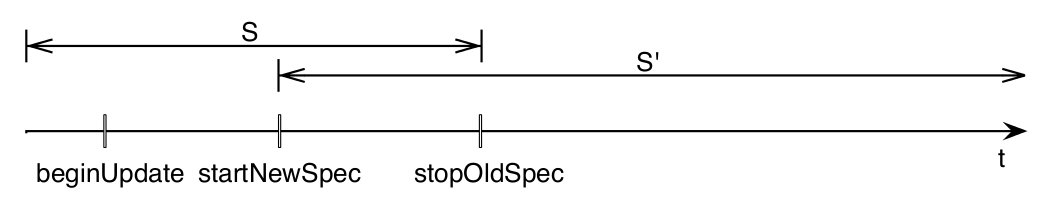
\includegraphics[scale=0.35]{img/overlaping.png}
\caption{Abstracción de la linea de tiempo de la actualización dinámica de controladores. Escenario en el cual la nueva
especificación está garantizada antes de que la vieja especificación deje de valer.}
\label{overlaping}
\end{figure}

\begin{figure}
\centering
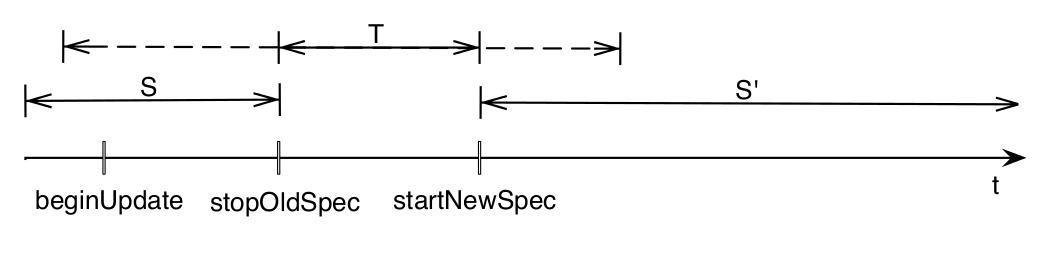
\includegraphics[scale=0.35]{img/transition.png}
\caption{Abstracción de la linea de tiempo de la actualización dinámica de controladores. Escenario en el cual hay un
periodo donde ni la vieja, ni la nueva especificación vale.}
\label{transition}
\end{figure}

Según nuestro conocimiento, el primer y único trabajo que investiga sobre actualización dinámica de controladores donde
hay un cambio de especificación explícito es en Ghezzi et al. \cite{6224401}. Ellos adoptan un criterio general,
natural y correcto. Una actualización dinámica es correcta si el comportamiento exhibido por el sistema es equivalente
al obtenido luego de una actualización apagando la máquina. Esto relaja el esfuerzo del ingeniero al no tener que
especificar requerimientos de transición (como en nuestro trabajo) pero con el costo de limitar posibles actualizaciones
que pueden ser soportadas. Como en \cite{6224401}, permitimos especificaciones solapadas (ver Figura \ref{overlaping}); pero
también permitimos periodos en los que ninguna especificación vale a diferencia de \cite{6224401} (ver Figura
\ref{transition}).

Es posible obtener el comportamiento de actualización obtenido en \cite{6224401} especificando como parte del
requerimiento de transición $T$ que $startNewSpec$ pueda ocurrir si la nueva especificación vale desde el último estado
inicial antes de $beginUpdate$ (ver la imagen de abajo de la Figura \ref{ghezzi}) o tan pronto como el estado inicial es
alcanzado nuevamente (ver la imagen de arriba de la Figura \ref{ghezzi}). Esto, podemos formalizarlo de la siguiente manera:

\vspace{-1cm}
\begin{equation}
\label{ghezzi_formula}
\Box [(LastInitBeforeUpdate \wedge G'\ W\ startNewSpec) \lor (startNewSpec \Longrightarrow Init)]
\end{equation}
\noindent donde $LastInitBeforeUpdate = Init \wedge \bigcirc(\neg Init\ W\ beginUpdate)$ y $Init$ representa estar en un estado inicial de
$C$.


\begin{figure}
\centering
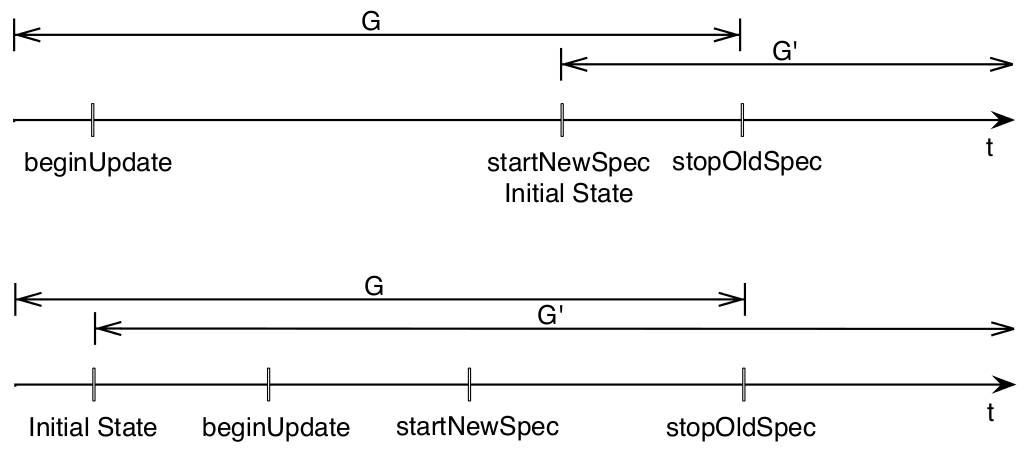
\includegraphics[scale=0.35]{img/Ghezzi.png}
\caption{Relación de eventos relevantes en la actualización de controladores dinámicamente para estados actualizables
según \cite{6224401}}
\label{ghezzi}
\end{figure}

En \cite{PanzicaLaManna:2013:FCC:2487336.2487349}, tres criterios de actualización mas débiles son introducidos para
permitir actualizaciones en sistemas donde el estado inicial no es visitado nuevamente. Por ejemplo, la noción de
estados co-inicial (estados que son similares al estado inicial), expande las situaciones en las cuales la actualización
es permitida. De todos modos, no hay garantías, para ninguno de los nuevos criterios, que el criterio correcto original
si tiene. La falta de garantías requiere de un ingeniero que valide el controlador resultante. En nuestro trabajo,
involucramos a un ingeniero capacitado y habilitado para proveer una especificación de un criterio correcto para la
actualización ($T$).

